\documentclass[a4paper,11pt]{article}
\usepackage[utf8]{inputenc}
\usepackage{amstext}
\usepackage{amssymb}
\usepackage{jcappub} % for details on the use of the package, please
                     % see the JCAP-author-manual

\usepackage[T1]{fontenc} % if needed

\usepackage[utf8]{inputenc}
\usepackage{graphicx}
\usepackage{float}
\usepackage{subfigure}
\usepackage{color}


% Local defines
\def\d{{\mathrm{d}}}
\def\beq{\begin{equation}}\def\eeq{\end{equation}}
\def\bea{\begin{eqnarray}}\def\eea{\end{eqnarray}}
\def\hateq{\mathop{\widehat{=}}}
\newfont{\cursive}{pzcmi at 9pt}


\title{Residuals of the gravitational wave events GW151012, GW151226 and GW170104}
\author[a]{Felicia Frederiksson,\note{Corresponding author.}}
\author[b]{Paolo Marcoccia,}
\author[b]{Alex B. Nielsen}

% The "\note" macro will give a warning: "Ignoring empty anchor..."
% you can safely ignore it.

\affiliation[a]{University of Uppsala, Uppsala, Sweden}
\affiliation[b]{University of Stavanger, Stavanger, Norway}


\abstract{%
Using methods previously develpoed we examine the residuals for the three gravitational wave events GW150914,GW151012, GW151226, GW170104.}

\begin{document}

\maketitle

\section{Introduction}

\subsection{Background about gravitational waves}
The detection of gravitational waves by LIGO was a major milestone in the history of astronomy.

Einstein's theory of general relativity is the standard paradigm for gravity. This has been well tested in the Solar Systems and passed with flying colours. Gravitational wave observations can be used to test the theory in new environments, particularly the merger of black holes. Black hole mergers are currently unobservable by other techniques, so all observational data currently comes from gravitational waves alone. A robust analysis of the gravitational wave data is thus of key importance.

Without a specific model of what deviations from general relativity would look like, one can ask the more restricted question of whether the data is compatible with the predictions of general relativity. One way to do this is to examine whether there is residual signal that is not explained by general relativity.

\subsection{Background about doubts}
Doubts were raised about the LIGO analysis in \cite{Creswell:2017rbh}. Some of these issues were addressed in the work of \cite{Nielsen:2018bhc}, focusing on the first, and to date loudest binary black hole event, GW150914. Here we extend this investigation to the other events discussed in \cite{Creswell:2017rbh}, namely GW151226 and GW170104 and the other event from the first observing run GW151012.

The authors of \cite{Creswell:2017rbh} write that a clear distinction between signal and noise has yet to be established for the contribution of gravitational waves.

\subsection{Introduction of methodology}

We adopt here a method similar to the one of \cite{Nielsen:2018bhc}. We subtract from the gravitational wave strain data a theoretical modeled signal and look for correlations in the resulting residuals. We apply this method to the first four events of LIGO, GW150914, GW151012, GW151226 and GW170104. Only the case of GW150914 was discussed in \cite{Nielsen:2018bhc}. While the concerns of \cite{Creswell:2017rbh} focussed mainly on GW150914, they also claimed that similar issues arose for GW151226 and GW170104. They did not discuss at all GW151012. Here we analyse all four of these results, which were the only events known at the time of \cite{Creswell:2017rbh}. Further LIGO events could be analysed in a similar way, both those already detected and those that will be detected in the future.

We do some things differently from \cite{Nielsen:2018bhc}. In particular we chose to whiten the data rather than bandpass and notch the data. This simplifies our analysis, allowing this choice to be applied to all events equally. It also more closely follows the practice in the wider gravitational wave literature. We apply a varying frequency bandpass to each event. This is in part determined by the inferred properties of the signal and thus is not a valid choice for a truly blind search for new signals. We take the approach that our unblind analysis acts as a sanity check of events found by other methods.

We produce a background for each of our events using simulated, uncorrelated Gaussian noise. We do this for each event, taking into account the different features of the analysis for each event.

To understand the relationship between the correlation statistic computed here and the detection statistics computed from matched filtering, in addition to studying actual events, we also study an number of simulated events using known signals of known parameters. This allows us to examine how the correlation statistic varies as the total mass and luminosity distance of the source are varied and gives an indication of what might be expected for other events not studied here. 

\section{Methodology}

Here we largely follow the methodology of \cite{Nielsen:2018bhc} and adapt their online codes, but extend to other LIGO events GW151012, GW151226 and GW170104. Extending to these different events means that we are forced to make some changes relative to what was done in \cite{Nielsen:2018bhc}. 

We use the maximum likelihood waveforms produced by the method described in \cite{Biwer:2018osg}. This reference contains results for the events of the first observing run. Results for all the events of the second observing run can be found in \cite{De:2018zrk}.

Several choices need to be made in presenting the results. A bandpass, a time offset between detectors and a waveform template to subtract. The choices for GW150914 in \cite{Creswell:2017rbh} were adapted from the somewhat arbitrary choices made to produce  Figure 1 of \cite{Abbott:2016blz}. The same choices were then used in \cite{Nielsen:2018bhc}. For the other events, there is no correspondence to Figure 1 of \cite{Abbott:2016blz} and so other possibilities must be sought. 

\section{GW150914}

The results for GW150914 were discussed in detail in \cite{Nielsen:2018bhc}. We give here some extended results for ease of comparison with the other events that are discussed below.

\begin{figure}[]
  \centering
    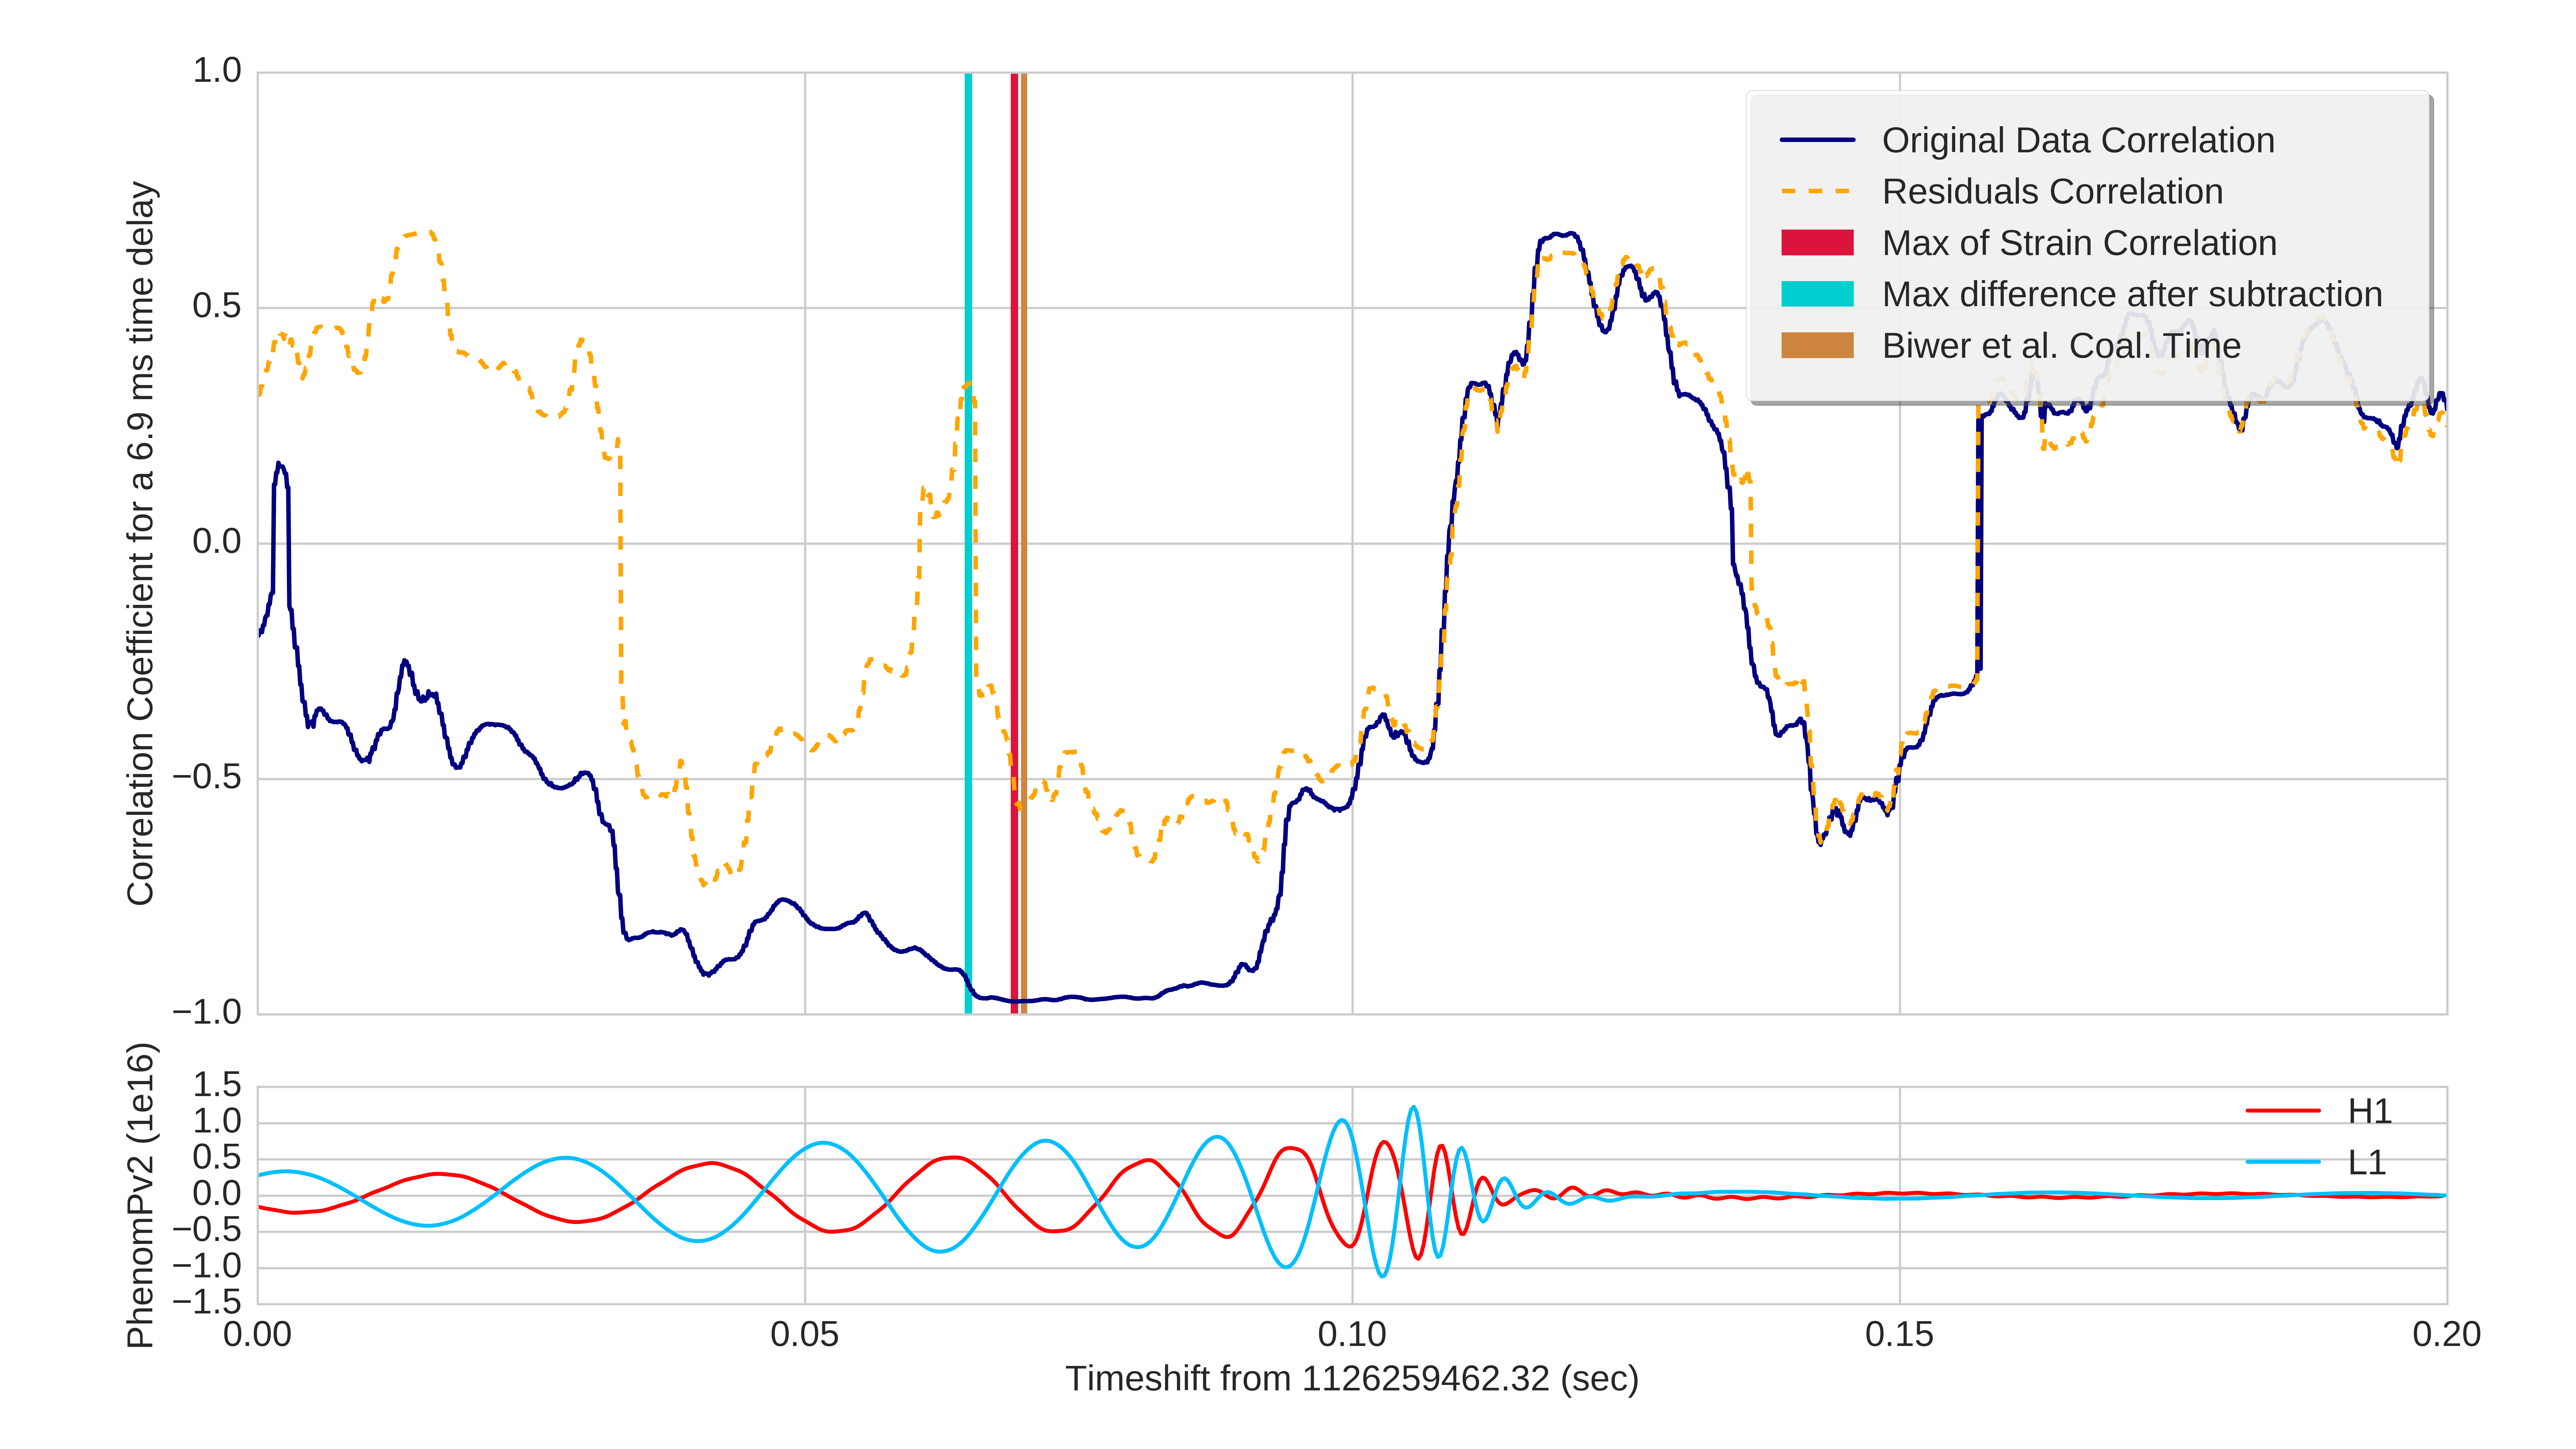
\includegraphics[width=\columnwidth]{GW150914CorrVsTime.png}
\caption{Correlations between H and L detector data for 200 ms of data around GW150914}
\label{fig:150914corr}
\end{figure}

In \cite{Jackson:2019xbq} it is noted that for the residual GW150914 analysis of \cite{Nielsen:2018bhc}, the maximum negative peak correlation of the entire time range from -10ms to +10ms, still lies in the grey band for the approximate time offset between the two detectors. This effect is a key contributor to the claim in \cite{Jackson:2019xbq} that the residual correlations of \cite{Nielsen:2018bhc} are still statistically significant. Here we see that whitening the data and choosing an event time of the maximal correlation, there is no longer a global negative peak in the grey region, there is only a local positive peak. The existence or not of a peak in the residual is not robust to different choices in the analysis method, whereas the peak for the full data is robust to this change.

\section{GW151012}

\begin{figure}[]
  \centering
   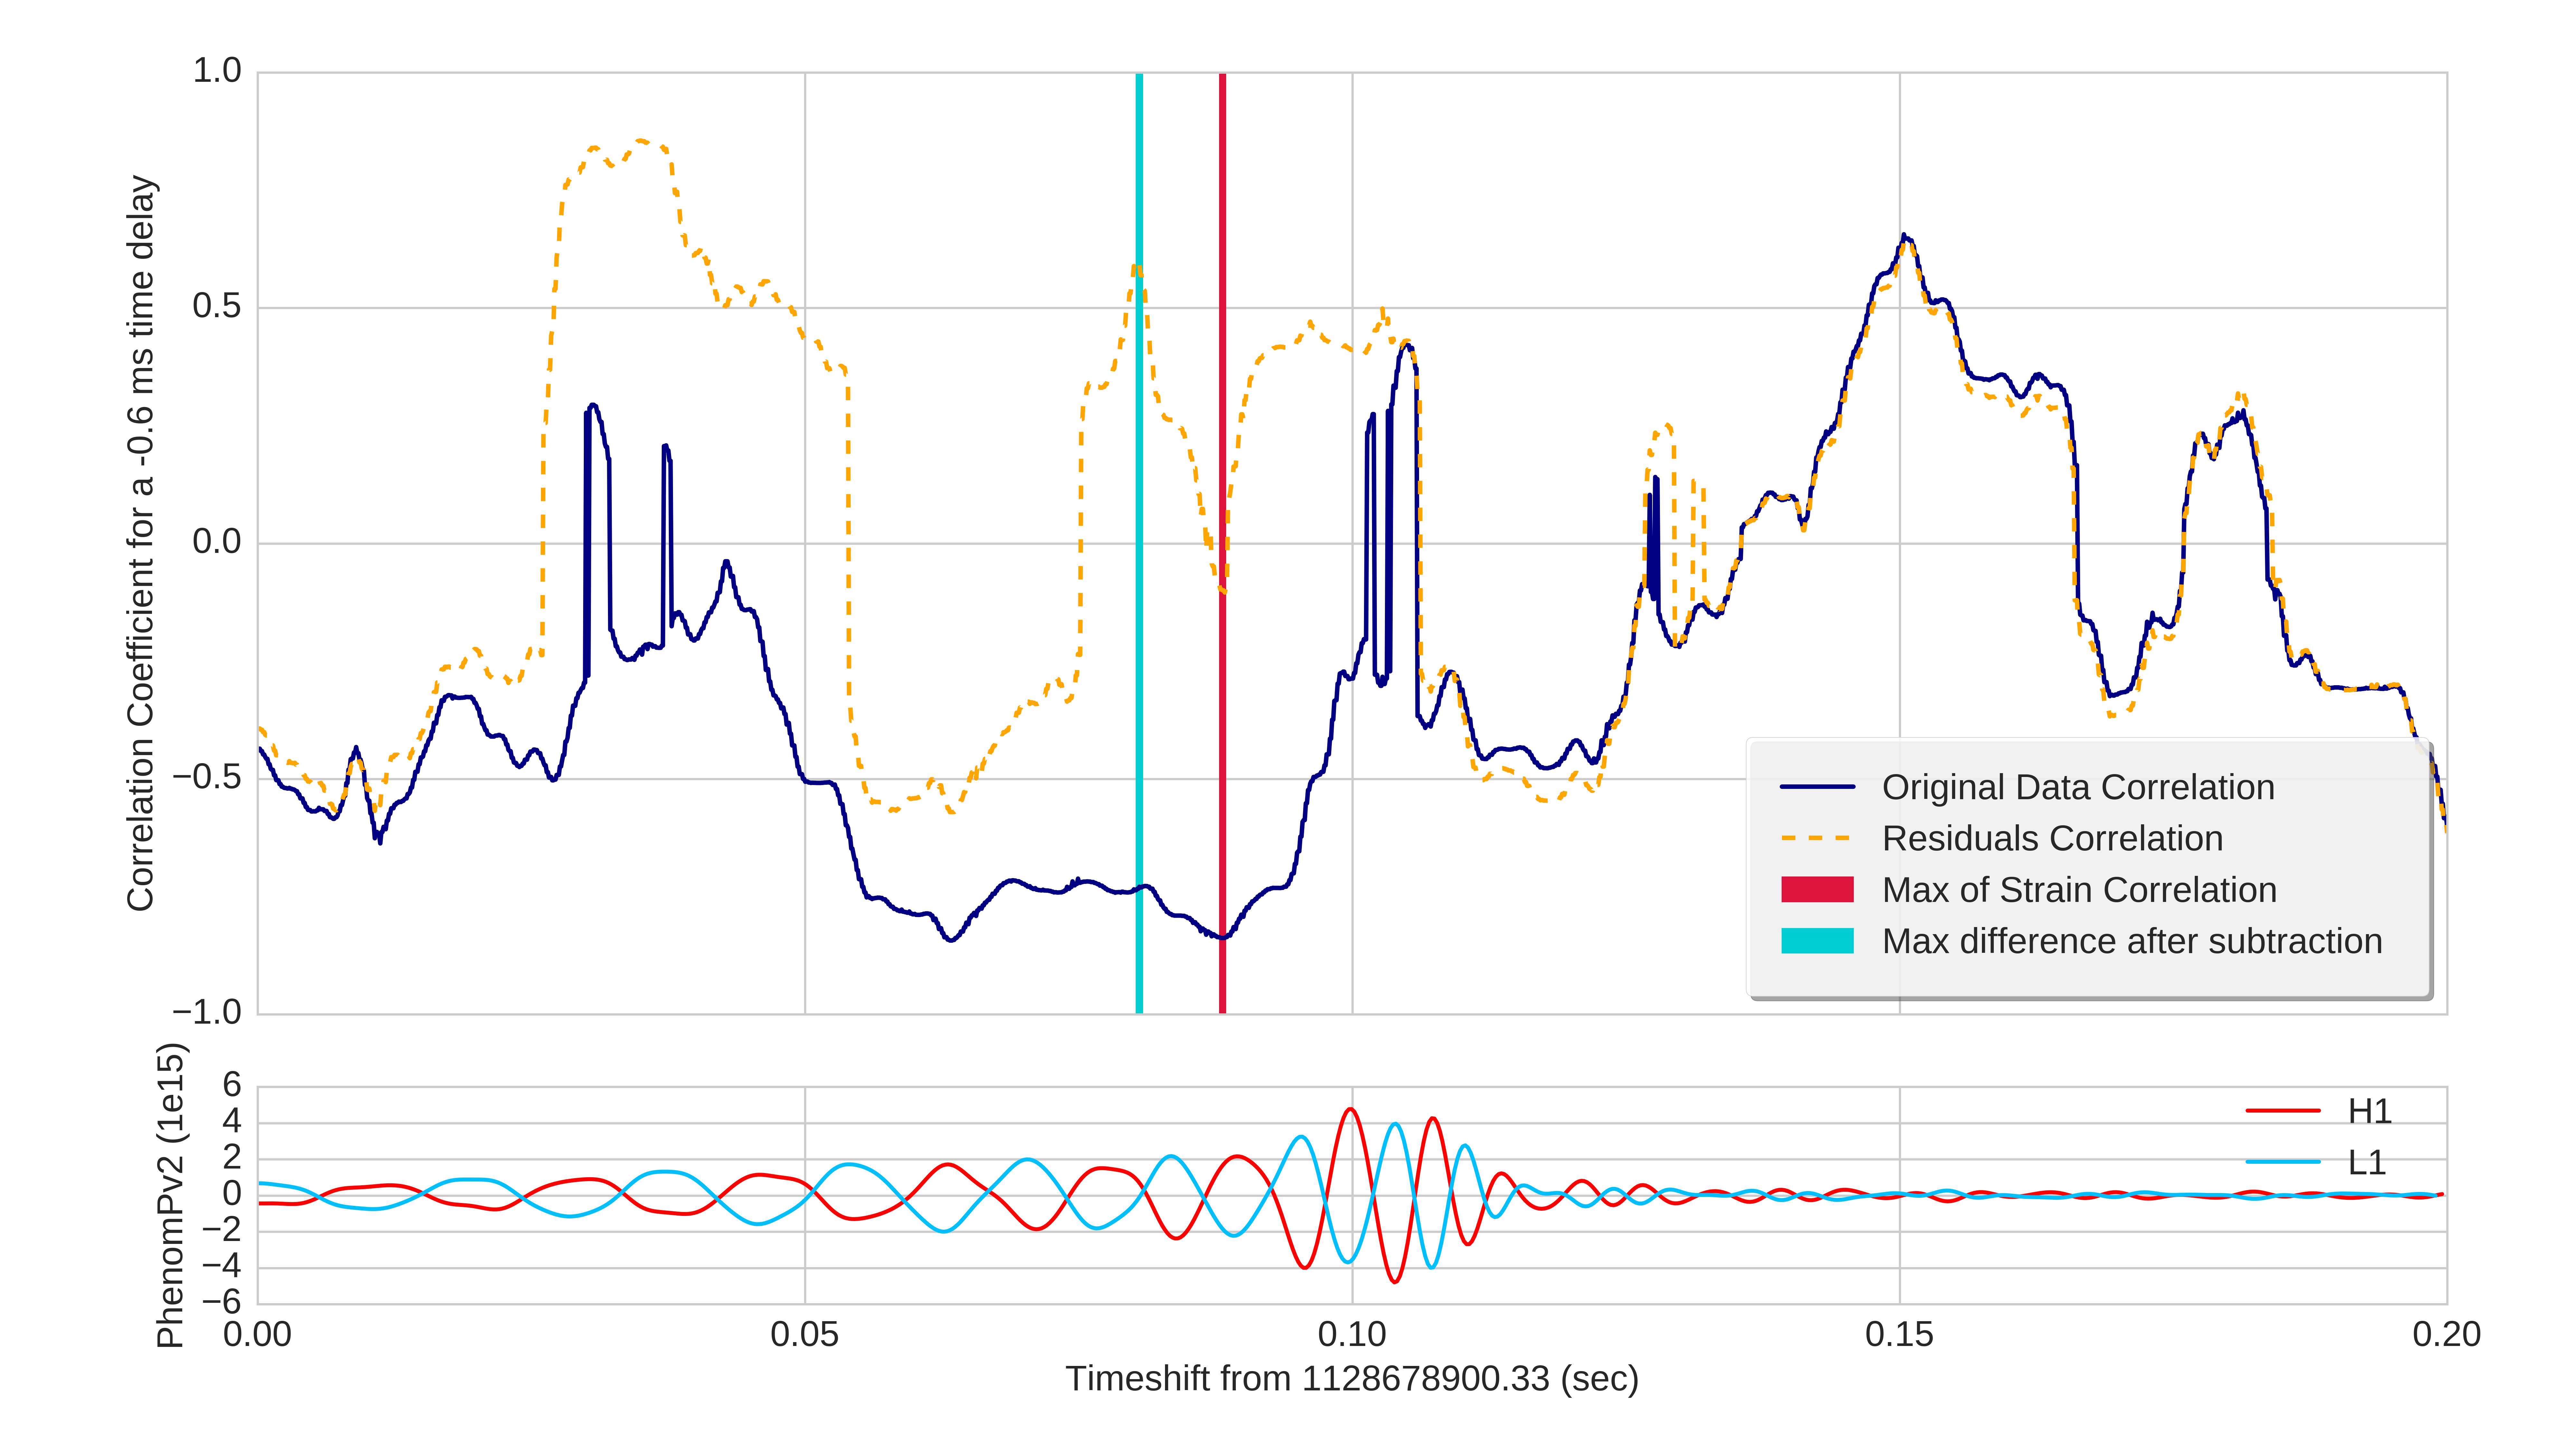
\includegraphics[width=\columnwidth]{GW151012CorrVsTime.png}
\caption{Correlations between H and L detector data for 200 ms of data around GW151012}
\label{fig:151012corr}
\end{figure}

\section{GW151226}

\begin{figure}[]
  \centering
    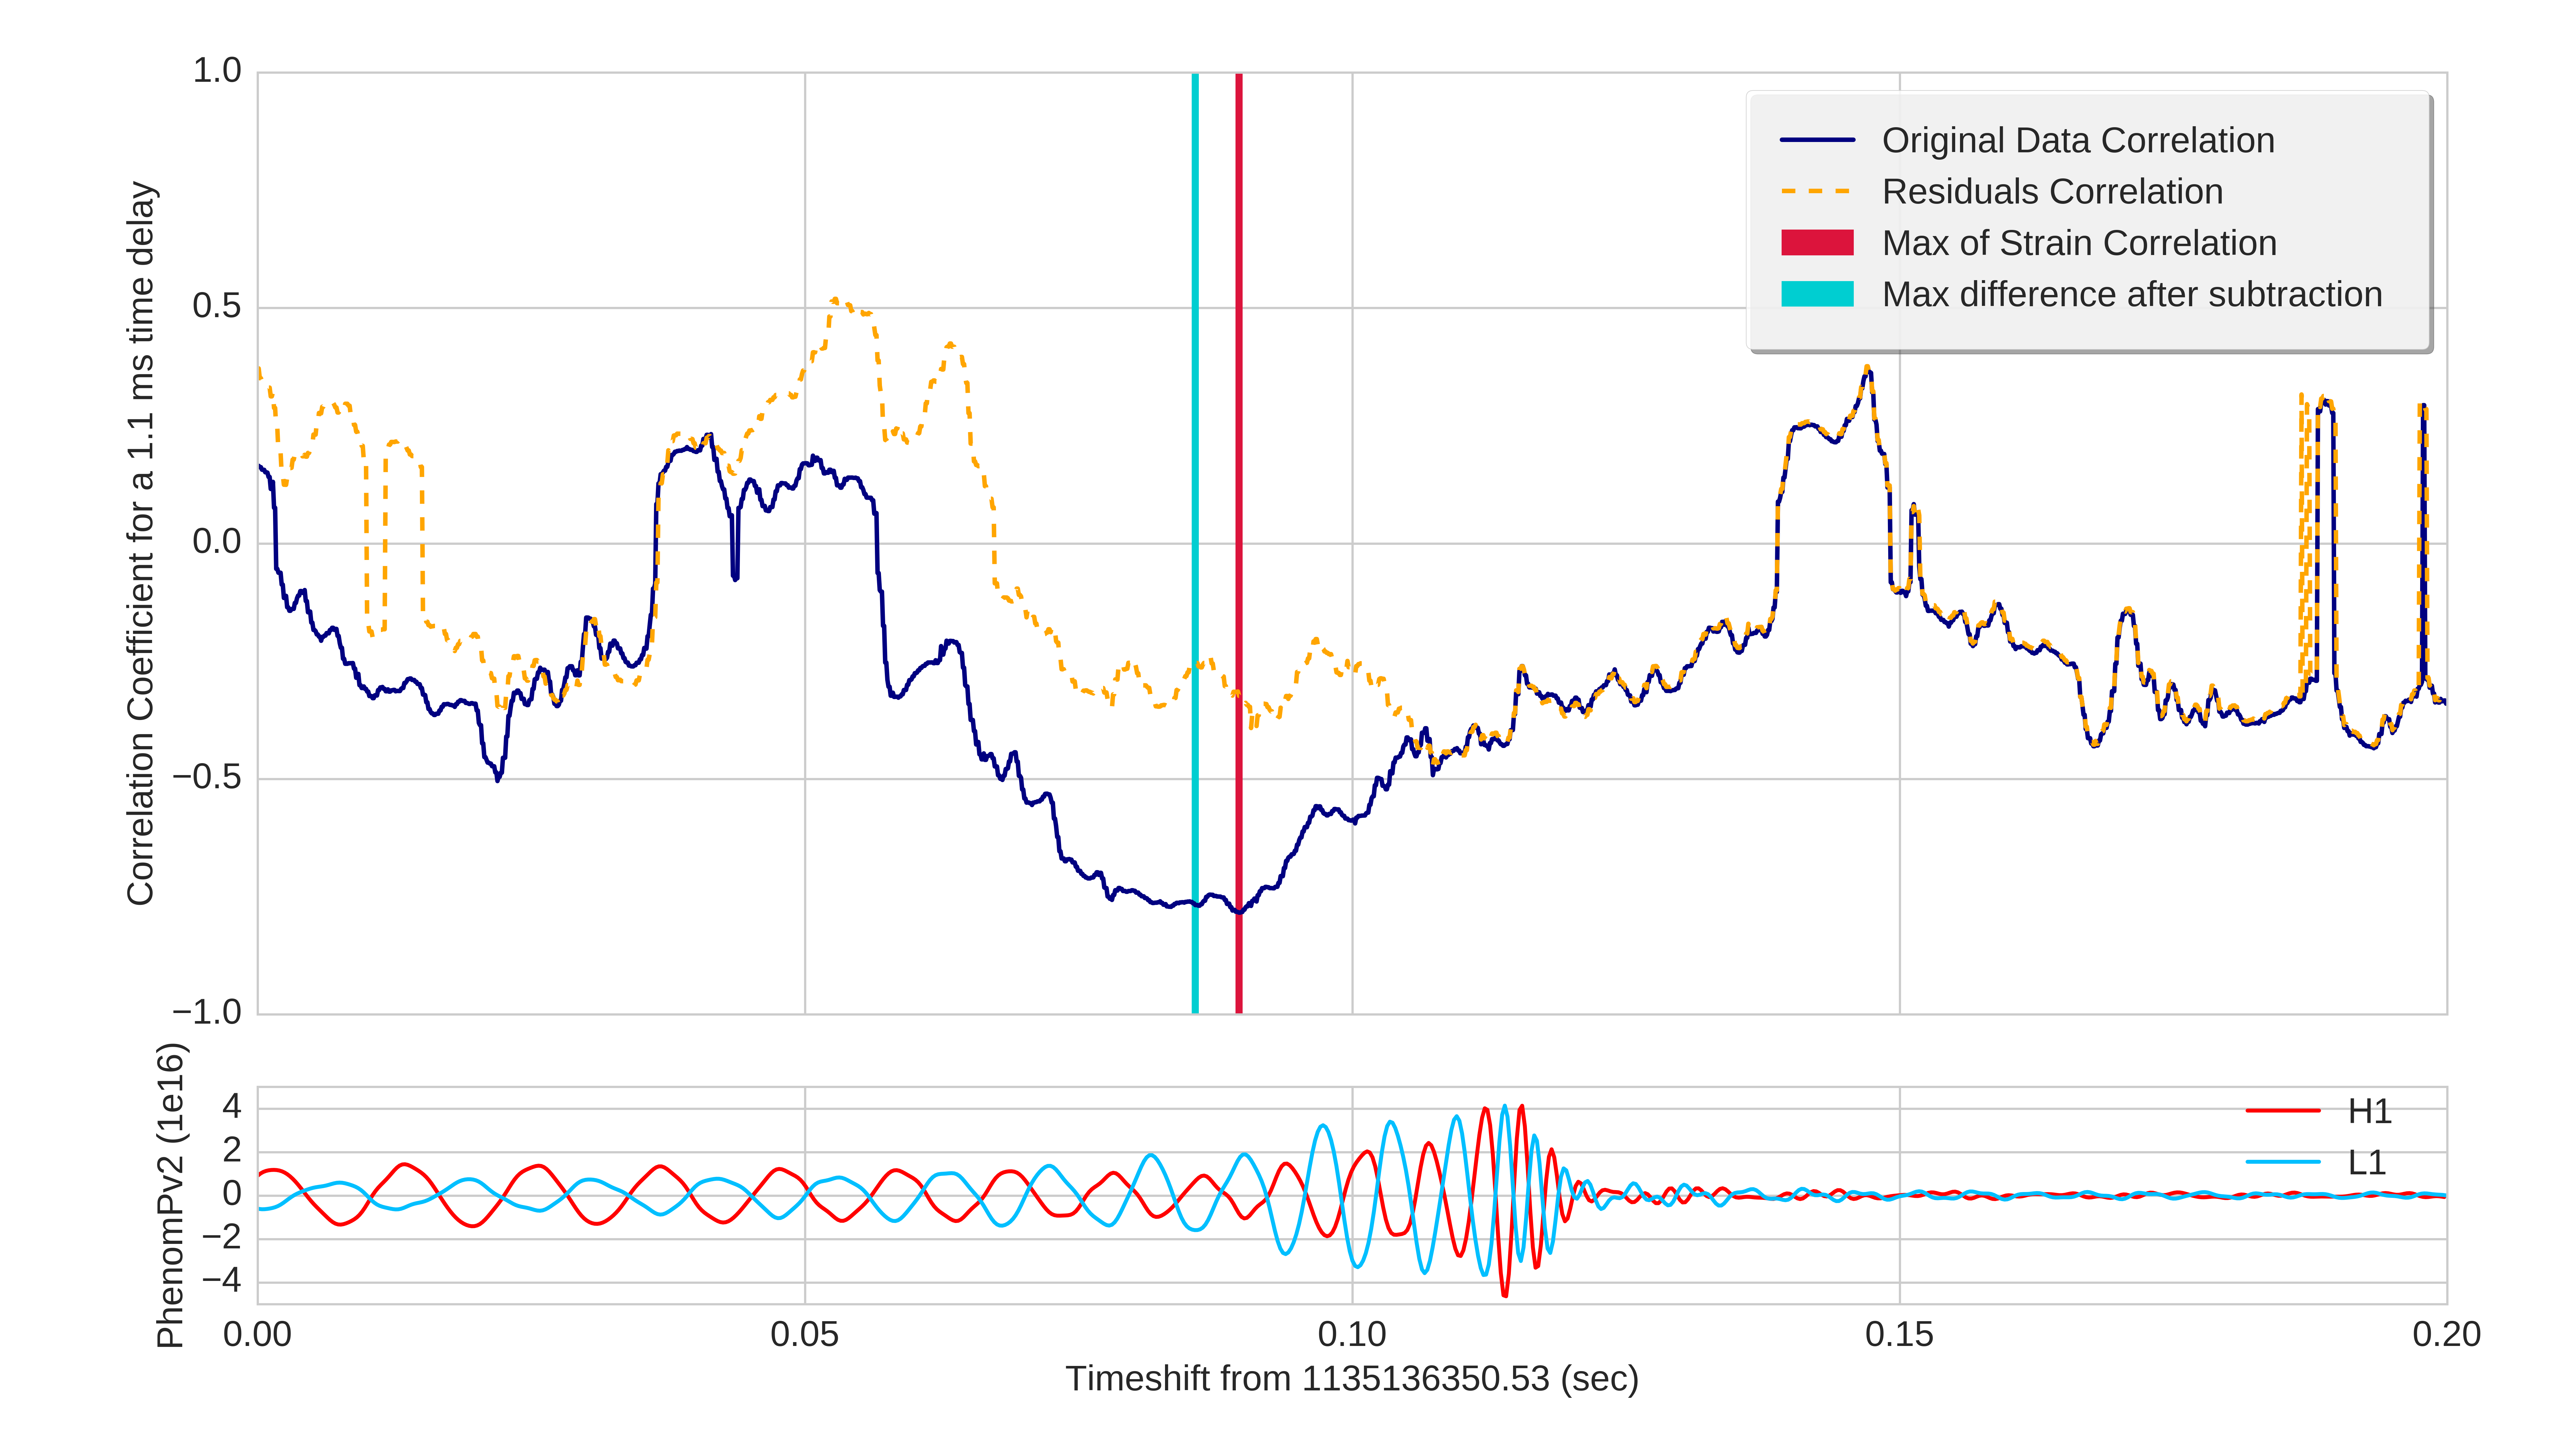
\includegraphics[width=\columnwidth]{GW151226CorrVsTime.png}
\caption{Correlations between H and L detector data for 200 ms of data around GW151226}
\label{fig:151226corr}
\end{figure}


\section{GW170104}

\begin{figure}[]
  \centering
    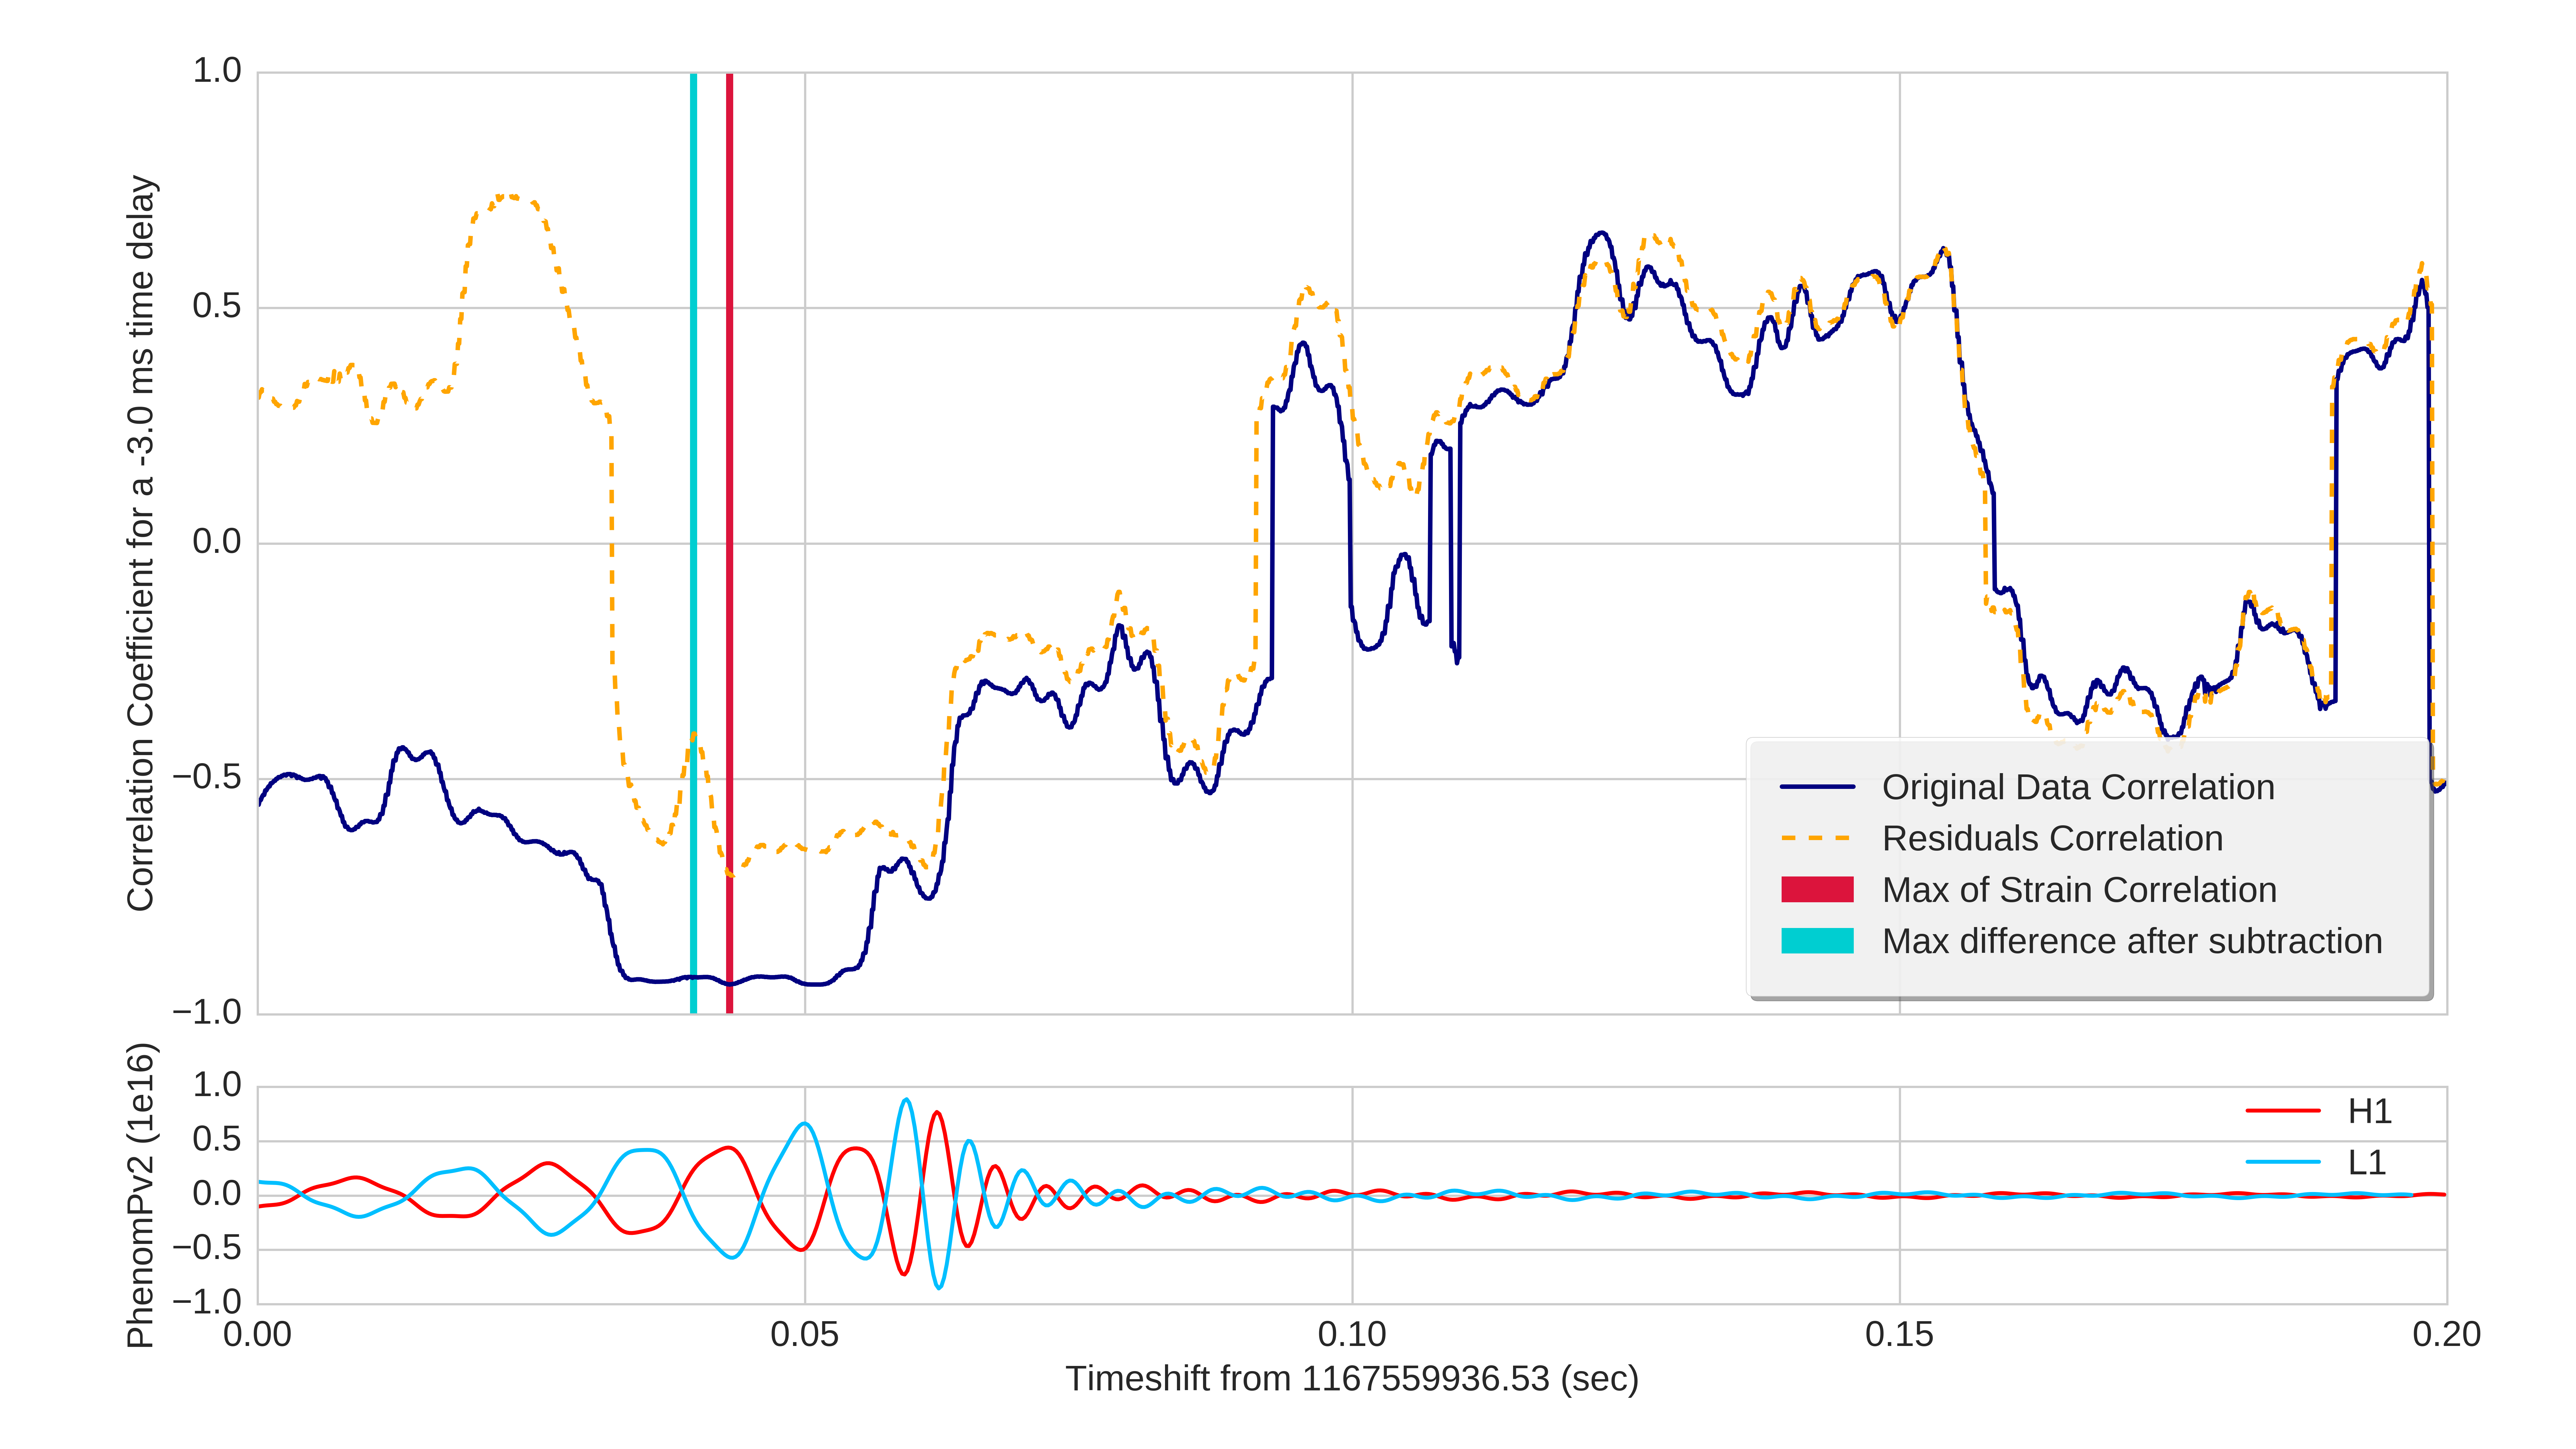
\includegraphics[width=\columnwidth]{GW170104CorrVsTime.png}
\caption{Correlations between H and L detector data for 200 ms of data around GW170104}
\label{fig:170104corr}
\end{figure}

\section{Backgrounds and statistical meaning of the result}

To summarize, we'll show the correlation at the time of the max, in function of the time shift between the detectors, for all the previously described events.

\begin{figure}[]
  \centering
    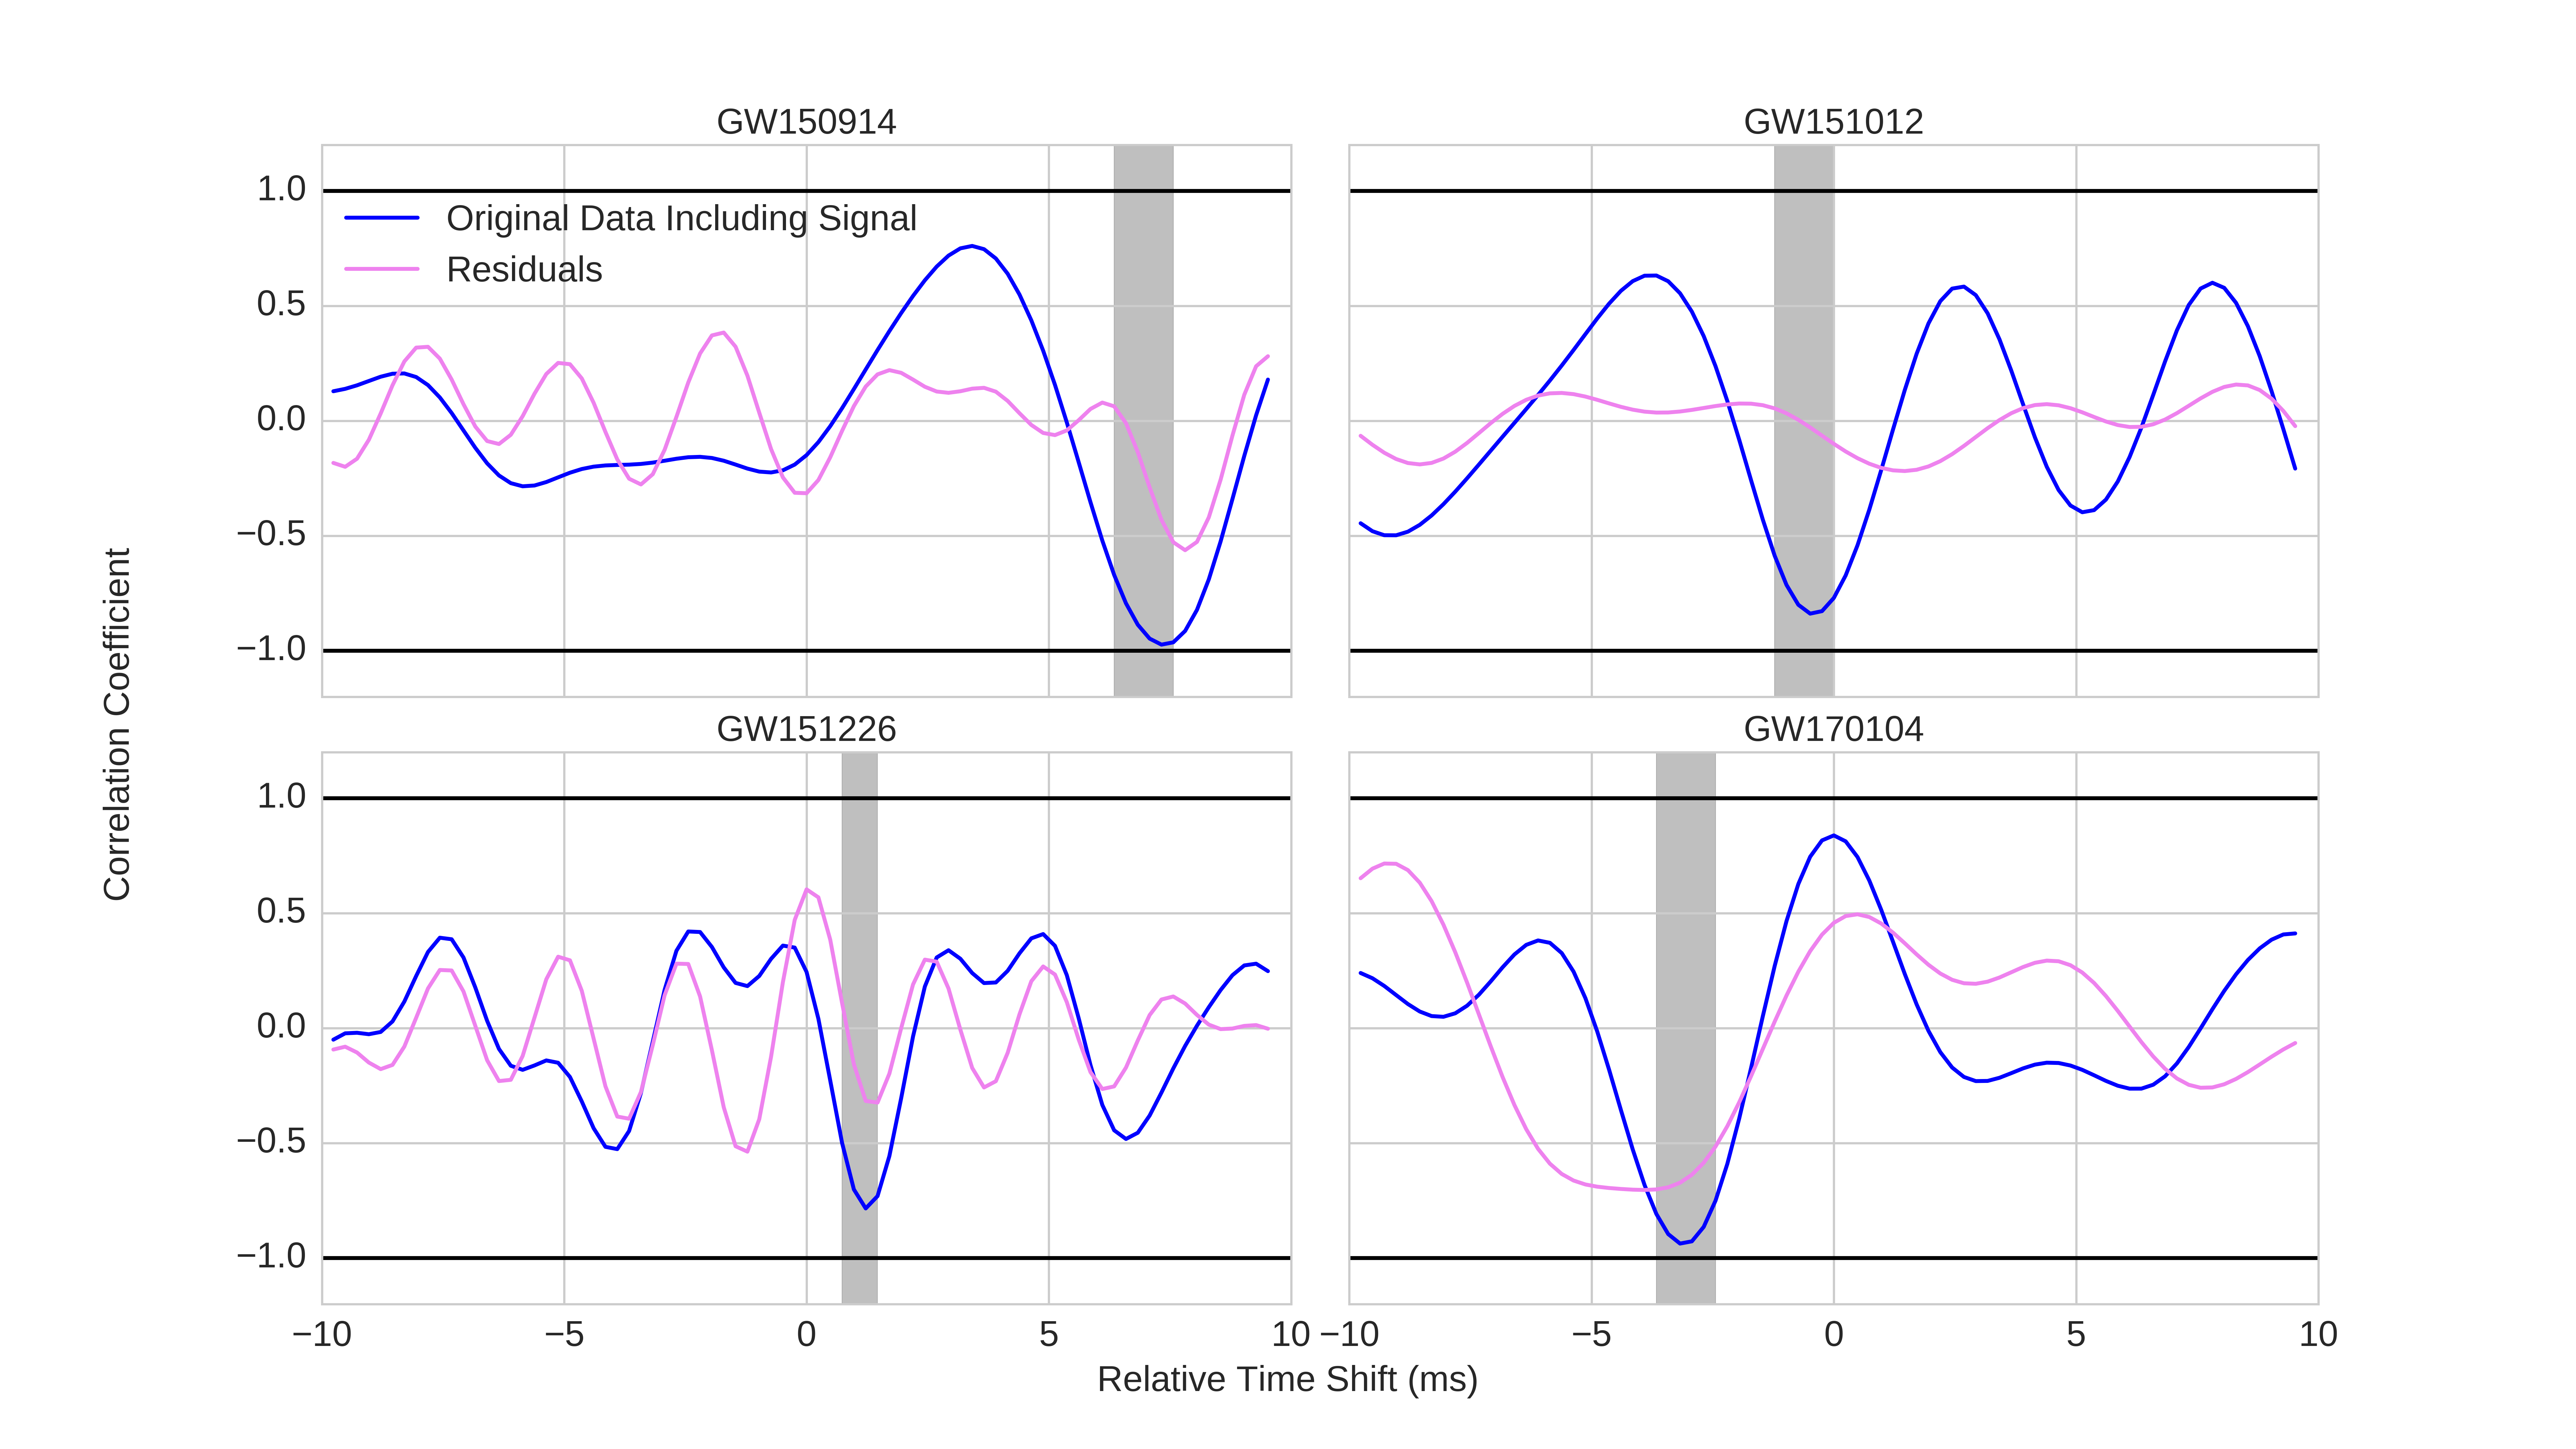
\includegraphics[width=\columnwidth]{AllMaxCorrVsTimeShift.png}
\caption{Correlations between H and L detector data, in function of the time shift, for the 4 events at the time of the Maximum.}
\label{fig:CorrVsTimeShift}
\end{figure}

We now have to express correlations in terms of their statistical meaning, to do so, we have run a correlation analysis on the background, i.e. at a time far away from any known events, and we estimated the frequencies of the values of correlations between the detectors, in function of the frequency range used for the whitening. From the number of occurrences of the correlation values among pure noise, we could express the values obtained for the correlations of our events, both in terms of pure strain and residuals, in terms of probability. The comparation between the backgrounds and the correlation values are shown in the following figure.

\begin{figure}[]
  \centering
    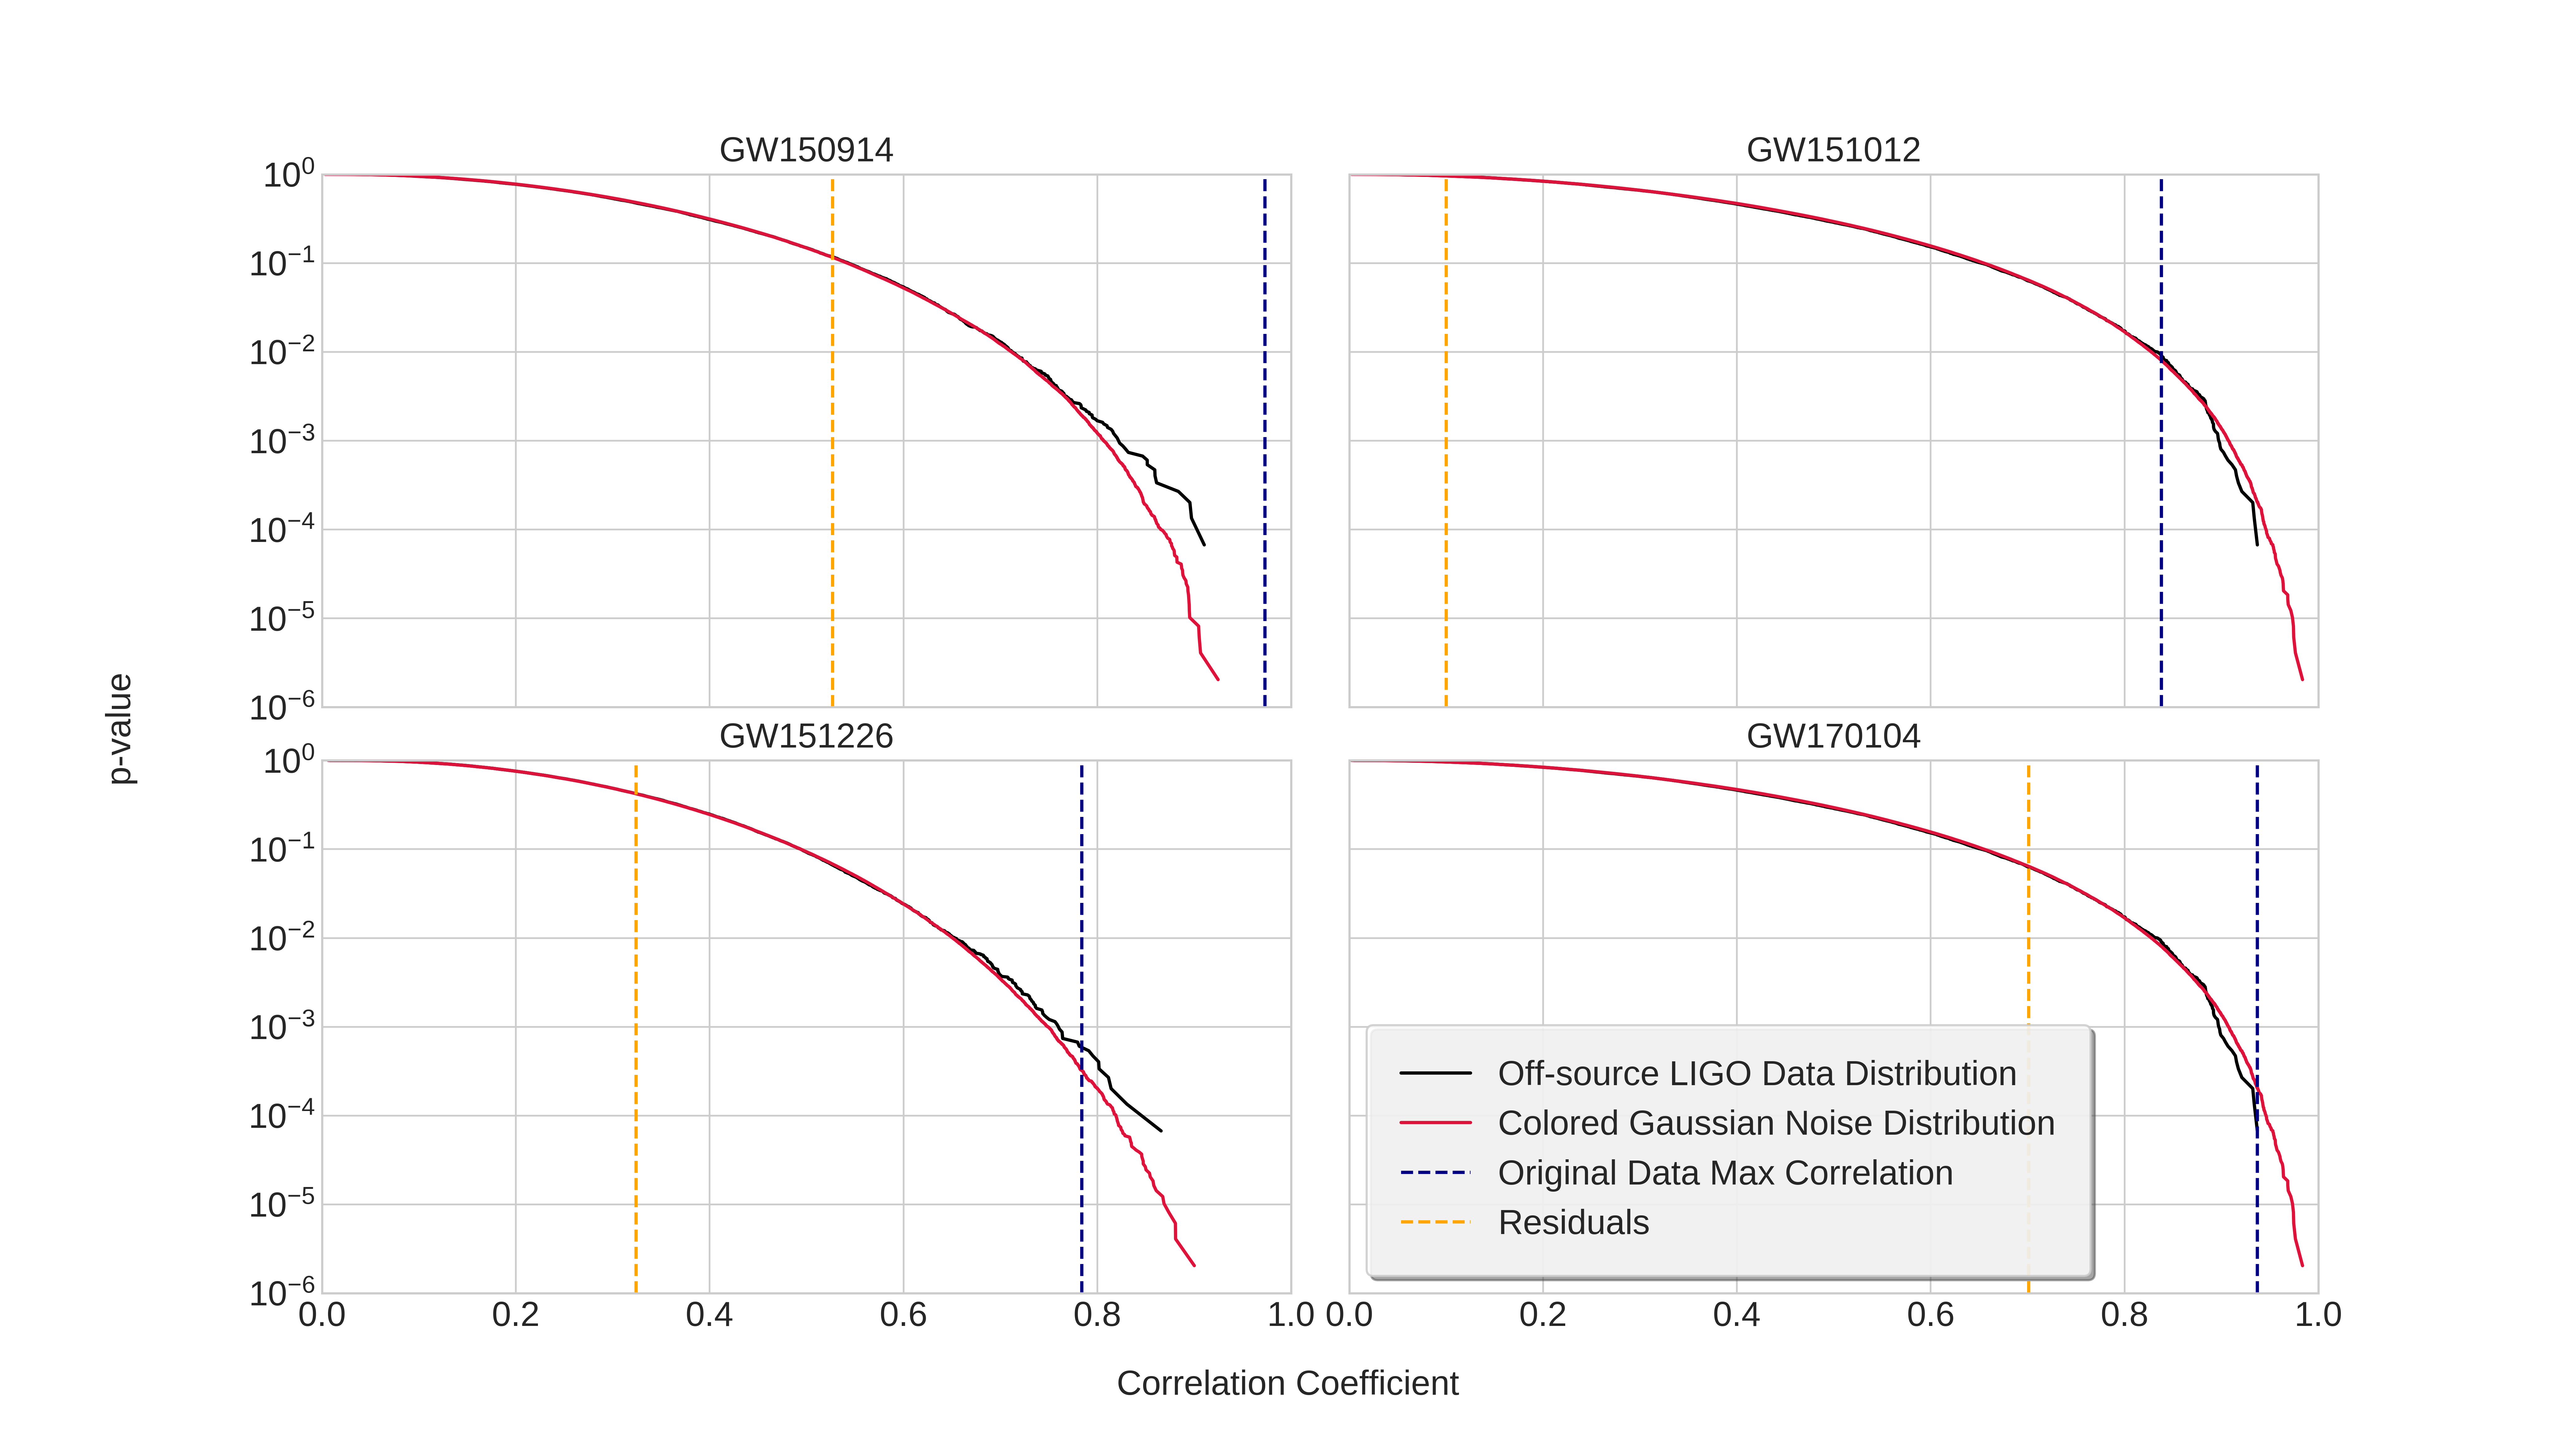
\includegraphics[width=\columnwidth]{AllBackgrounds.png}
\caption{Comparation between the correlation values obtained for the events, and their occurrences in pure noise.}
\label{fig:Backgrounds}
\end{figure}

\section{References}
\begin{thebibliography}{9}

%\cite{Abbott:2016blz}
\bibitem{Abbott:2016blz}
  B.~P.~Abbott {\it et al.} [LIGO Scientific and Virgo Collaborations],
  %``Observation of Gravitational Waves from a Binary Black Hole Merger,''
  Phys.\ Rev.\ Lett.\  {\bf 116} (2016) no.6,  061102
  doi:10.1103/PhysRevLett.116.061102
  [arXiv:1602.03837 [gr-qc]].

%\cite{Biwer:2018osg}
\bibitem{Biwer:2018osg}
  C.~M.~Biwer, C.~D.~Capano, S.~De, M.~Cabero, D.~A.~Brown, A.~H.~Nitz and V.~Raymond,
  %``PyCBC Inference: A Python-based parameter estimation toolkit for compact binary coalescence signals,''
  Publ.\ Astron.\ Soc.\ Pac.\  {\bf 131} (2019) no.996,  024503
  doi:10.1088/1538-3873/aaef0b
  [arXiv:1807.10312 [astro-ph.IM]].

%\cite{Creswell:2017rbh}
\bibitem{Creswell:2017rbh}
  J.~Creswell, S.~von Hausegger, A.~D.~Jackson, H.~Liu and P.~Naselsky,
  %``On the time lags of the LIGO signals,''
  JCAP {\bf 1708} (2017) no.08,  013
  doi:10.1088/1475-7516/2017/08/013
  [arXiv:1706.04191 [astro-ph.IM]].

%\cite{De:2018zrk}
\bibitem{De:2018zrk}
  S.~De, C.~M.~Biwer, C.~D.~Capano, A.~H.~Nitz and D.~A.~Brown,
  %``Posterior samples of the parameters of binary black holes from Advanced LIGO, Virgo's second observing run,''
  Scientific Data 6, 81 (2019)
  doi:10.1038/s41597-019-0086-6
  [arXiv:1811.09232 [gr-qc]].

%\cite{Jackson:2019xbq}
\bibitem{Jackson:2019xbq}
  A.~D.~Jackson, H.~Liu and P.~Naselsky,
  %``Noise residuals for GW150914 using maximum likelihood and numerical relativity templates,''
  JCAP {\bf 1905} (2019) no.05,  014
  doi:10.1088/1475-7516/2019/05/014
  [arXiv:1903.02401 [astro-ph.IM]].

%\cite{Maroju:2019ymy}
\bibitem{Maroju:2019ymy}
  R.~Maroju, S.~R.~Dyuthi, A.~Sukrutha and S.~Desai,
  %``Looking for ancillary signals around GW150914,''
  JCAP {\bf 1904} (2019) no.04,  007
  doi:10.1088/1475-7516/2019/04/007
  [arXiv:1903.02823 [astro-ph.IM]].

%\cite{Nielsen:2018bhc}
\bibitem{Nielsen:2018bhc}
  A.~B.~Nielsen, A.~H.~Nitz, C.~D.~Capano and D.~A.~Brown,
  %``Investigating the noise residuals around the gravitational wave event GW150914,''
  JCAP {\bf 1902} (2019) 019
  doi:10.1088/1475-7516/2019/02/019
  [arXiv:1811.04071 [astro-ph.HE]].
  

\end{thebibliography}


\end{document}